%%=============================================================================
%% Methodologie
%%=============================================================================

\chapter{\IfLanguageName{dutch}{Methodologie}{Methodology}}
\label{ch:methodologie}

%% TODO: Hoe ben je te werk gegaan? Verdeel je onderzoek in grote fasen, en
%% licht in elke fase toe welke stappen je gevolgd hebt. Verantwoord waarom je
%% op deze manier te werk gegaan bent. Je moet kunnen aantonen dat je de best
%% mogelijke manier toegepast hebt om een antwoord te vinden op de
%% onderzoeksvraag.

\section{Inhoud}

Allereerst worden de \textbf{empirische tests} uitgevoerd. Deze tests gaan na of de digitalisatie mogelijk is op technisch vlak. Het doel van dit onderzoek is analoge apparatuur om te vormen in pure software zodat het toegankelijker is voor consumenten met een lager budget. Daarom werd voor de technische tests gebruik gemaakt van een standaard particulieren laptop. De code geschreven voor de uitvoering van de tests wordt samen met de specificaties van het testsysteem respectievelijk besproken in secties \ref{subsec:methodologie:code} en \ref{subsec:methodologie:testmachine}.

Zodat de testcases van de empirische tests representatief zouden zijn, werd er gezocht naar real-life usecases uit de muzieksector. Hiervoor zijn interviews afgenomen. De interviews zelf zijn besproken in sectie \ref{sec:interviews}. In de interviews werden artiesten, producers etc. gevraagd naar hun opstellingen voor zowel in opname als voor live muziek. Aan hand van die informatie werden representatieve testcases opgesteld. De opstelling van de testcases staan uitgelegd in sectie \ref{subsec:methodologie:code}. 

In de interviews werd ook gevraagd of digitale varianten verwelkomd zouden worden op de markt. Dit is interessant voor software bedrijven die de muzieksector willen betreden. Als er wel degelijk vraag is naar zulke innovaties, weten zij dat het voordelig is om in die niche te gaan werken. Hoe de antwoorden van de interviewees verwerkt werden staat beschreven in sectie \ref{sec:methodologie:emotioneletests}. Dit zijn de \textbf{emotionele tests}.

\section{Empirische tests}
\label{sec:methodologie:empirischetests}

\subsection{De Testmachine}
\label{subsec:methodologie:testmachine}

Er werd gezocht naar een laptop met gemiddelde specificaties voor de hedendaagse markt. Als deze laptop de testcases al aankan dan geldt hetzelfde voor andere gemiddelde particuliere laptops en zeker voor workstations van opnamestudio's en backstage geluidstechnici.

De gekozen machine is een Lenovo Ideapad Flex-14. Het modelnummer is 20308. De specificaties van de machine staan in tabel \ref{tab:specmachine}. Op de machine draaide een verse installatie van Linux Mint Sylvia.

\begin{table}[]
\centering
\begin{tabular}{lll}
\hline
\multicolumn{3}{c}{\textbf{Component}}                \\ \hline
\textbf{Type} & \textbf{Naam}       & \textbf{Kracht} \\ \hline
Processor     & Intel Core i3-4010U & 1.70GHz         \\ \hline
RAM           & DDR3L SDRAM         & 8,00 GB         \\ \hline
Opslag        & Hybride Drive       & 500 GB
\end{tabular}
\caption{Specificaties van de Testmachine}
\label{tab:specmachine}
\end{table}

\subsection{De Code}
\label{subsec:methodologie:code}

\subsubsection{Keuze en Werking van de Libraries}

Uit de interviews, besproken in sectie \ref{sec:interviews}, bleek dat de muzieksector altijd met subtractive synthesis werkt bij hun geluidsgeneratie en -verwerking. Voor de empirische tests zijn dus drie subtractive sound synthesis libraries gekozen. Zoals vermeld in sectie \ref{sec:libraries} zijn dit Beads, JASS en JSyn.

Sectie \ref{subsec:vergelijkinglibraries} toont aan dat de drie libraries in essentie een gelijkaardige werking hebben. Iedere oscillator en geluidsverwerkende klasse voert een specifieke bewerking uit op een buffer. De buffers kunnen ook aan elkaar geconnecteerd worden; de output van de buffer wordt de input van een andere. Zo maakt de gebruiker een stramien van parameters die hij kan gebruiken om het geluid te modeleren.

\subsubsection{Opstelling van de Testcases}

De testcases zijn opgesteld aan de hand van de interviews. De interviewees werden gevraagd naar volgende specificaties van hun opstelling. 

\begin{itemize}
	\item Hoeveel audiosporen er gebruikt worden.
	\item Op hoeveel van die sporen equalization en compressie van toepassing is.
	\item Het aantal effecten dat op eenzelfde moment actief is op een spoor.
	\item Op hoeveel van die sporen het stramien van effecten actief staat.
	\item Hoeveel parameters ze op één moment moeten bedienen.
\end{itemize}

Het aantal sporen werd in code vertaald naar oscillatoren. Die oscillatoren werden geconnecteerd aan equalizers en compressors. Die output werd - indien van toepassing - ook geconnecteerd aan een stramien van effecten. Alle losse outputs van oscillatoren, compressors en effecten werden aangesloten op de audio output lijn van het programma. Op die manier konden de antwoorden weergegeven worden als volgende vier integere parameters.

\begin{itemize}
	\item Het aantal oscillatoren.
	\item Het aantal oscillatoren dat geconnecteerd wordt aan een equalizer en compressor.
	\item Het aantal effecten.
	\item Het aantal oscillatoren dat - eventueel na hun connectie aan een compressor - aan een stramien van effecten geconnecteerd wordt.
\end{itemize}

Voor het opstellen van de testcases is rekening gehouden met hoeveel buffers berekend worden in het programma. De testcases worden per library uitgevoerd in stijgende volgorde van het aantal gebruikte buffers. De paramerters staan per profiel weergegeven in tabellen \ref{tab:profielen} en \ref{tab:parameters}.

\begin{table}[]
\begin{tabular}{ll|c}
\textbf{Interviewee} & \textbf{Profiel} & \textbf{Testcase index} \\ \hline
- & Hobbyist & 1 \\
Vagabundos \& Peter Boone & Live band & 2 \\
Vagabundos \& Peter Boone & Band in opname & 3 \\
Saulo Soneghet & Metal band in opname & 4 \\
Bart Vincent & Jazz band in concert & 5 \\
Thomas Houthave & Sound designer & 6 \\ \hline
\end{tabular}
\caption{Testcase index per profiel}
\label{tab:profielen}
\end{table}

\begin{table}[]
\begin{tabular}{c|cccc|c}
\textbf{Index} & \textbf{\#Tracks} & \textbf{\#EQ en compressie} & \textbf{\#Effecten} & \textbf{\#Tracks met effecten} & \textbf{\#Buffers} \\ \hline
1 & 4 & 4 & 0 & 0 & 4 \\
2 & 10 & 10 & 2 & 5 & 40 \\
3 & 25 & 25 & 2 & 10 & 95 \\
4 & 40 & 40 & 3 & 15 & 165 \\
5 & 50 & 50 & 5 & 20 & 250 \\
6 & 150 & 150 & 0 & 0 & 450 
\end{tabular}
\caption{Testcase parameters per index}
\label{tab:parameters}
\end{table}

\subsubsection{Architectuur en Werking van de Test Framework}
\label{subsub:testframework}

De code voor het uitvoeren van de testcases is terug te vinden in appendix \ref{ch:code}.

De volgende taak was om een test framework te maken. Met de parameters geformuleerd in tabel \ref{tab:parameters}, moet het framework library-specifieke testcases uitvoeren en de performantie meten van het proces. Er werd rekening gehouden met uitbreidbaarheid zodat andere libraries makkelijk toegevoegd kunnen worden. Daarvoor werd de template pattern toegepast.

\begin{figure}
  \centering
    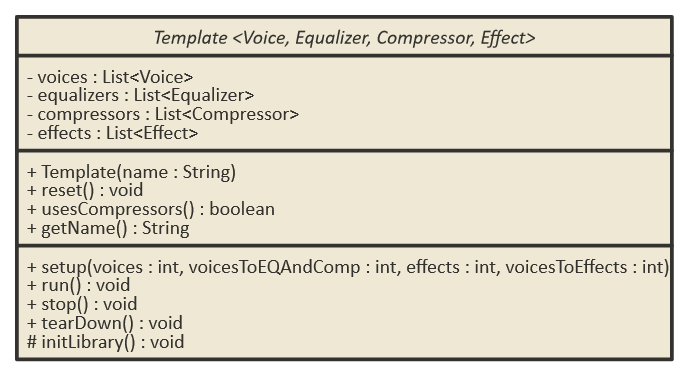
\includegraphics[width=0.5\textwidth]{imgs/nomnoml.png}
  \caption{Klasse diagram van de Template klasse}
  \label{fig:template}
\end{figure}

Figuur \ref{fig:template} toont het klasse diagram van de abstracte en generieke \verb+Template+ klasse van het framework. Dit is de moederklasse van de library specifieke testklasses. Wanneer een klasse zich uitbreid op \verb+Template+, representeert de subklasse een sound synthesis library. De subklasse moet eerst de generieke types \verb+Voice+, \verb+Equalizer+, \verb+Compressor+ en \verb+Effect+ definiëren.

\begin{itemize}
	\item \textbf{Voice} is een oscillatorklasse uit de library.
	\item \textbf{Equalizer} is een klasse uit de library die een inkomende buffer verwerkt. Om trouw te blijven aan de real-life testcases gebruikt men hier best een geluidsfilter. Geluidsfilters hebben karakteristieken van equalizers.
	\item \textbf{Compressor}: idem aan \textbf{Equalizer}.
	\item \textbf{Effect} is nog een verwerkende klasse. Deze klasse representeert een geluidseffect. Bart Vincent en Vagabundos gebruikten vaak een delay effect. \autocite{bartvincent} \autocite{vagabundos} Het wordt aangeraden om een gelijkaardig effect uit de library te kiezen.
\end{itemize}

 In de subklasse worden vervolgens de \verb+setup+-, \verb+run+-, \verb+stop+- en \verb+tearDown+-methode overgeërft. Deze worden als volgt ingevuld.

\begin{itemize}
	\item \textbf{Setup} vraagt de vier parameters uit tabel \ref{tab:parameters}. Aan de hand van deze parameters worden de \verb+Voice+-, \verb+Equalizer+-, \verb+Compressor+-, \verb+Effect+-modules correct geïnstantieerd, geconnecteerd en opgeslagen in de desbetreffende attributen uit de \verb+Template+-klasse.
	\item De \textbf{run}-methode start alle oscillatoren en verwerkende modules die in de \verb+setup+-methode opgesteld zijn. Sound synthesis libraries starten in de meeste gevallen automatisch een nieuwe thread wanneer dit gebeurt. Als dit niet het geval is, moet de ontwikkelaar het zelf in een thread laten uitvoeren\footnote{JASS start bijvoorbeeld geen nieuwe thread wanneer SourcePlayer.start() opgeroepen wordt. Om dit op te lossen werd de PlayThread-klasse ontworpen die de SourcePlayer eenmalig start tot de halt methode opgeroepen wordt.}. Dit is belangerijk voor de performantiemeting. 
	\item De \textbf{stop}-methode stopt de thread - en bijgevolg ook het geluid - die in de \verb+run+-methode opgeroepen is.
	\item \textbf{TearDown} haalt de opstelling van de testcase terug uit elkaar. Voor de modules verwijderd kunnen worden uit het geheugen, moeten ze eerst veilig gedeconnecteerd worden van zowel de library als van de andere componenten. Zo kan de library terug volledig geïnitialiseerd worden voor de volgende testcase.
\end{itemize}

De uit te voeren testklassen en de parameters van de testcases worden statisch bijgehouden in de \verb+StartUp+-klasse. In de \verb+main+-methode wordt per testklasse iedere testcase uitgevoerd. Tijdens het runnen van de audio thread, wordt de performantie van het proces gemeten.

\subsubsection{Performantiemeting van het Proces}

Het voordeel van in een Linux-omgeving te werken is dat er geen externe library nodig is voor de performantiemeting. Alle nodige informatie kan al verkregen worden via het \verb+top+-commando. De taak voor het afnemen van de metingen werd in het framework aan de \verb+Measurer+-klasse gegeven. In die klasse kan commando \ref{command} teruggevonden worden.

\begin{figure}
\centering
\begin{verbatim}
	top -b -n1 -d,01 | \\
	grep %d | \\
	awk '{ if (\$9 != \"0,0\") print \$9 \" \" \$10 }'
\end{verbatim}
\caption{Linux commando om performantie van een proces te meten.}
\label{command}
\end{figure}

\verb+Top+ is een real-time commando. Wanneer het opgeroepen wordt in de terminal, worden alle processen en hun verbruik van CPU en geheugen dynamisch weergegeven. \autocite{topcommand} De volgende vlaggen worden toegepast.

\begin{itemize}
	\item \textbf{-b} start het proces in \textit{Batch mode}. Dit zorgt dat de header met algemene infromatie niet afgebeeld wordt zodat de output beter verwerkt kan worden door andere programma's of commando's.
	\item \textbf{-n1} maakt maar één meting in plaats van een continue dynamische output te geven.
	\item \textbf{-d,01} voert de meting op 0,01 seconden uit.
\end{itemize}

De \verb+-n+-vlag wordt gebruikt omdat Java geen output van dynamische commando's kan lezen. De \verb+-d+-vlag wordt gebruikt zodat de enkele meting zo snel mogelijk gemaakt wordt. Zo doende dook er een probleem op. Wanneer \verb+top+ standaard uitgevoerd wordt, update het proces ongeveer iedere de seconde. Wanneer men de metingen frequenter uit voert, wordt vastgesteld dat de meting voor \verb+%CPU+ onleesbaar is. Ongeveer iedere seconde wordt er een geldige meting afgebeeld. Daartussen vertoont de meting een \verb+0+ als resultaat.

Het interval van de seconde is niet betrouwbaar; soms was het meer, soms was het minder. Daarom wordt iedere 0,01 seconden een meting genomen. Ongeldige metingen worden genegeerd door het programma. Andere metingen worden opgeslaan tot er een totaal van 50 metingen per testcase is. Iedere meting duurt nog steeds ongeveer een seconde, maar van het moment dat een geldige meting verkrijgbaar is, wordt die ook opgenomen. 

De output van het \verb+top+-commando wordt doorgegeven aan het \verb+grep+-commando. Java String formatting maakt gebruik van de \verb|"%d"| om de \textit{process ID} van het framework in te voeren in het commando. Zo verkrijgt men een enkele meting van het gezochte proces. \verb+StartUp+ heeft een statische methode \verb+getPID()+ die de \textit{process ID} van het framework teruggeeft. De output van \verb+grep+ wordt doorgegeven aan het \verb+awk+-commando.

Het \verb+awk+-commando filtert de \verb+%CPU+ en \verb+%Mem+ meting uit de output van \verb+grep+ op voorwaarde dat de \verb+%CPU+-meting geldig is. De output van dit commando wordt ingelezen door Java. De twee metingen worden nog gescheiden door een spatie zodat het makkelijk te verwerken is.

\subsection{Verwerking van de Testresultaten}
\label{sec:methodologie:verwerking}

Per library is er een dataset van 6 testcases. Iedere testcase heeft een subset van 50 metingen. Op zo'n subset wordt eerst een dubbele \textit{median three} smoothing uitgevoerd. \autocite{mediansmoothing} Dit is een smoothing methode waarbij twee keer een nieuwe dataset gemaakt wordt. De nieuwe dataset wordt bekomen door een item te vervangen door de mediaan van zichzelf, zijn voorganger en zijn nakomer; zoals getoond in berekening \ref{math:mediansmooth}. $y_{i}$ is het item van de nieuwe dataset en $x$ representeert de oude dataset. De eerste en laatste waarden worden overgenomen uit de oude dataset omdat berekening \ref{math:mediansmooth} niet mogelijk is op die indexen. Deze dubbele smoothing verwijdert korte periodes van extrema.

\begin{figure}
\centering
$y_{i} = med(x_{i-1}, x_{i}, x_{i+1})$
\caption{\textit{Moving median} formule}
\label{math:mediansmooth}
\end{figure}

De resulterende dataset wordt vervolgens gladgestreken door middel van de Hanning vensterfunctie. Deze functie maakt dat plotse variaties in het frequentiedomein geëgaliseerd worden. Op die manier komen waarden die frequenter voorkomen in de dataset dominanter naar voor. Dit door het lopend gewogen gemiddelde van de waarden in de dataset te berekenen. De Hanning van een waarde in een dataset wordt berekend als de helft van die waarde opgeteld met een kwart van de voorgaande en nakomende meting. Dit staat afgebeeld in berekening \ref{math:hanningformule}. De eerste en laatste waarden van de nieuwe dataset worden overgenomen uit de oude dataset. \autocite{hanning}

\begin{figure}
\centering
$h_{i} = (y_{i-1} + 2 \ast y_{i} + y_{i+1}) \div 4$
\caption{Hanning formule}
\label{math:hanningformule}
\end{figure}

Van de resulterende dataset wordt de mediaan genomen als resultaat voor de testcase. De mediaan is niet gevoelig aan extrema en geeft een betere representatie van de meer frequente metingen in een dataset. \autocite{median} Van de medianen wordt een trendlijn berekend. Zolang de richtingscoëfficient van de trendlijn van de testresultaten niet hoger ligt dan die van het aantal buffers in de input parameters uit tabel \ref{tab:parameters}, kunnen we zeggen dat het technisch aanvaardbaar is om een overstap naar digitaal te maken. 

\section{Emotionele tests}
\label{sec:methodologie:emotioneletests}

Na de technische bespreking van de muzikale opstellingen van de interviewees, werden volgende vragen gesteld:

\begin{itemize}
	\item Is er potentie voor digitalisering in de muziekindustrie?
	\item Wie zou hier het meeste baat bij hebben?
	\item Wie zou hier het meeste interesse in hebben?
	\item Zou een digitalisering verwelkomd worden in de sector?
\end{itemize}

Op basis van deze vragen, weten we of de branche van dat profiel in de muzieksector open staat voor een digitalisatie.

Er zijn door tijdsgebrek en de kleine respons (zie tabel \ref{table:correspondentie}) slechts vier interviews afgenomen. Dit is duidelijk te weinig data om een populatie te representeren. Alle interviewees spreken uit jaren vakkundige ervaring. Daarom kan hun antwoord waardevol in aanmerking genomen worden. 

Iedere interviewee beeld een profiel uit zoals in tabel \ref{tab:profielen} staat. Als resultaat op de emotionele test van een profiel wordt uit belang van dit onderzoek het resultaat van de interviewee zelf genomen.

\iffalse \lipsum[21-25] \fi

